\begin{frame}{Circuito 3: isolamento da carga com buffer}
  \small
  \begin{columns}[T,onlytextwidth]
    \begin{column}{0.48\textwidth}
      \centering
      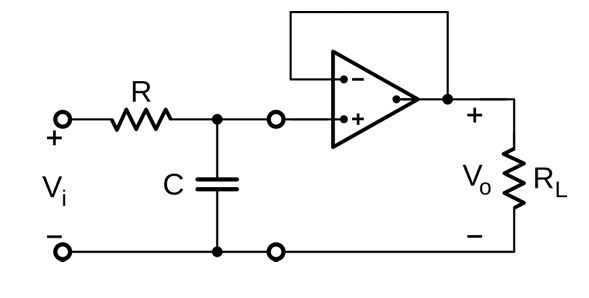
\includegraphics[width=\linewidth,height=0.27\textheight,keepaspectratio]{slides/img/circuito_3.png}

      \begin{block}{Modelo ideal do seguidor}
        $i^+=i^-=0$ e $v^-=v^+$.
        Como $v^-=V_o$, resulta $V_o=v^+$.
        \[
          \frac{V_i-v^+}{R}=sCv^+.
        \]
      \end{block}
    \end{column}
    \begin{column}{0.48\textwidth}
      \begin{alertblock}{Função de transferência restaurada}
        \[
          H_3(s)=\frac{1}{1+sRC}=H_1(s).
        \]
        \[
          K_3=1,\qquad f_{c3}=\frac{1}{2\pi RC}.
        \]
        No projeto nominal, $f_{c3}\approx48{,}23\,\mathrm{Hz}$.
        O valor de $R_L$ não entra na função de transferência ideal.
      \end{alertblock}
      A alimentação do ampop fornece a corrente de carga.
      O ganho de tensão do buffer é unitário.
    \end{column}
  \end{columns}
\end{frame}
